\documentclass[twoside]{article}


\usepackage[utf8]{inputenc}
\usepackage[T1]{fontenc}
\usepackage{lmodern}
\usepackage[english]{babel}
\usepackage{geometry}
\usepackage{booktabs}
\geometry{margin=1in}
\usepackage{setspace}
\usepackage{siunitx}
\usepackage{graphicx}
\usepackage{amsmath, amssymb}
\usepackage{array}
\usepackage{longtable}
\usepackage{fancyhdr}
\usepackage{hyperref}
\usepackage{float}

\hypersetup{
  colorlinks=true,
  linkcolor=black,
  filecolor=magenta,   
  urlcolor=blue,
  citecolor=blue,
  pdftitle={Investigating the Use of Agent-Based Modeling for Wildfire Prevention},
  pdfauthor={Kai Speidel},
  pdfsubject={Cognitive Science \& Artificial Intelligence Thesis},
  pdfkeywords={agent-based modeling, wildfire, simulation, drone swarms, firefighting},
  bookmarksnumbered=true,
  bookmarksopen=true,
  bookmarksopenlevel=1,
  pdfstartview=Fit,
}

\usepackage{bookmark}
\usepackage{natbib}


\usepackage{titlesec}
\titleformat{\section}{\normalfont\bfseries}{\thesection.}{1em}{}
\titleformat{\subsection}{\normalfont\bfseries}{\thesubsection}{1em}{}


\begin{document}


% Title Page 
\begin{titlepage}
  \thispagestyle{empty}
  \begin{center}

    \vspace{2cm}
    
    {\LARGE\bfseries Investigating the Use of Agent-Based Modeling for Wildfire Prevention: A Simulation Study\par}
    
    \vspace{2cm}
    \large Name: Kai Speidel \\
    \textsc{Student number: U627621}

    \vspace{2cm}
    \small
    \textbf{THESIS SUBMITTED IN PARTIAL FULFILLMENT} \\
    \textbf{OF THE REQUIREMENTS FOR THE DEGREE OF} \\
    \textbf{BACHELOR OF SCIENCE IN COGNITIVE SCIENCE \& ARTIFICIAL INTELLIGENCE} \\
    \textbf{DEPARTMENT OF COGNITIVE SCIENCE \& ARTIFICIAL INTELLIGENCE} \\
    \textbf{SCHOOL OF HUMANITIES AND DIGITAL SCIENCES} \\
    \textbf{TILBURG UNIVERSITY}

    \vspace{2cm}

    \large\textbf{Thesis Committee:} \\
    \normalsize
    Supervisor: Dr. Travis J. Wiltshire \\
    Second Reader: Natalie Ranzhi Wei, Msc. 

    \vfill

    Tilburg University \\
    School of Humanities and Digital Sciences \\
    Department of Cognitive Science \& Artificial Intelligence \\
    Tilburg, The Netherlands \\
    May 2025
  \end{center}
\end{titlepage}
\setcounter{page}{1}

\pagestyle{fancy}
\fancyhf{} % clear all header and footer fields
\fancyhead[LE]{\small Kai Speidel}     
\fancyhead[RE]{\small\nouppercase{\rightmark}}

% Odd pages (right-hand side)
\fancyhead[LO]{\small Cognitive Science \& Artificial Intelligence}
\fancyhead[RO]{\small 2025} 
\fancyfoot[C]{\thepage}


\begin{abstract}
Wildfires pose a growing threat resulting from climate change, the loss of biodiversity and human activity \citep{copernicus-wildfires}. This research explores economic and sustainable firefighting approaches using autonomous drone swarms, traditional aircraft, and hybrid models. A simulation framework created in Python using the agent-based modeling library Mesa \citep{terMesa} simulates these methods focusing on cost, environmental impact, and computational efficiency. Drones, planes, fires, and resource stations were modeled as agents in the environment with parameters supported by current research. Results from 1000 steps over 1000 simulation iterations prove that drone swarms significantly and consistently outperform manned aircraft in both sustainability and cost. Hybrid systems offer the fastest response but with higher emissions and costs. This research contributes an open-source framework for evaluating aerial firefighting strategies, designed to support evidence-based guidelines and encourage sustainable and frugal fire management.
\end{abstract}

\section{Data Source, Ethics, Code, and Technology (DSECT) Statement}
\label{sec:CodeOfCondunt}

\subsection{Data Source}

This thesis does not use any datasets or human/animal data. All data used in the project is synthetically generated through simulations developed by the author. No external data owners are involved, and no consent was necessary. All data was produced locally using custom agent-based models created in Python using the mesa library. The parameters of the simulation are taken from cited research.

\subsection{Figures}

All Figures, plots, tables and visualizations included in the thesis were created by the author using the original simulation output. No external or copyrighted images were used. Visuals were generated using Python libraries such as \texttt{matplotlib} and \texttt{seaborn}. The creation of the visuals is documented and explained in the GitHub repository \citep{AgentBasedFirefightingModel_repository}

\subsection{Code}

The simulation uses multiple open-source Python libraries such as \texttt{ mesa, numpy, pandas}, their implementation is documented in the Methodology section~\ref{sec:Methodology} and the referenced GitHub repository.

\subsection{Technology}

The thesis was typeset using the standard LaTeX thesis template provided by the university, with additional formatting packages such as \texttt{fancyhr, tikz} for formatting preferences. References were managed using BibTeX and LaTeX’s built-in bibliography environment. Zotero was used as a reference manager.
Generative models such as GitHub's Copilot, Claude and ChatGpt were used for harsh feedback on personal created text and code. The content was not directly copied; instead used as a valuable tool to generate feedback and point out room for improvement. All conceptual, experimental, and implementation work was done by the author, with inspiration from the documentation of the mentioned libraries.


\section{Introduction}
\label{sec:Introduction}

% - Why are wildfires problematic? 
% - How are they currently studied? 
% - What is ABM and why is it a powerful tool to study this phenomena? 
%- What are the components of your RQ that need to be explained? - Also see the results comment on RQs. 

Wildfires pose an escalating global threat, driven by climate change and human activity, with 96\% of wildfires being human-induced \citep{HybridAntColonyWildfire}. These events cause ecological, economic, and societal damage \citep{Saffre2022}, emitting over 2,000 megatons of carbon emissions globally in 2023 alone \citep{Lelis2024}. The UN Environment Program (UNEP2) forecasts a 50\% increase by the end of the century in extreme wildfires if no countermeasures are taken \citep{Sullivan2022}. Escalating wildfire frequency also threatens agricultural productivity \citep{IPCC2023} and poses significant health risks through smoke exposure \citep{Finlay2012}. These combined effects make wildfires one of the most urgent environmental and societal challenges today.

Wildfire research traditionally employs different methodological approaches with different advantages and limitations. Historical analysis creates the foundation of wildfire research. Researchers examine fire records, satellite imagery and climate data to identify patterns, trends and correlations between environmental factors and fire behavior \citep{copernicus-wildfires,IPCC2023}. These studies offer valuable insights into long-term fire cycles and climate relationship, but their retrospective nature limits their adaptability in the accelerating climate change. 

Field studies including controlled burns present another critical research approach \citep{wildland}. While these approaches offer scientists valuable real-world data about fire physics and suppression in a controlled environment, they are inherently limited by safety concerns, high costs and their impossibility of testing extreme scenarios or comparing multiple suppression strategies simultaneously.

Traditional aerial firefighting and data collection relies heavily on manned aircraft such as Helicopters or fixed-wing planes. For decades this has been the backbone of wildfire suppression \citep{janney2012airtankers}. These aircraft deliver water or fire retardant directly to the fire zones, often in dangerous conditions such as limited visibility. Their effectiveness comes with safety constraints, high operational cost and substantial carbon emissions \citep{spicerRapidMeasurementEmissions2009}.

Recent technological advancements have sparked growing interest in autonomous drone systems for wildfire suppression. Modern drone technology potentially offers operation in extreme conditions without risking human life while being lower in cost and emissions. Research done by \citet{Yan2024} effectively demonstrates the possibility of using coordinated swarm behavior to detect forest fires. Current research presents promising applications such as new suppression techniques like the ''fireball'' by \citet{fireBalls}.

While the development is promising especially with more applied drone applications being tested, scientists have also turned to simulation studies as they provide evidence for fire spread behavior at a lower cost. One of the earliest tools in this domain was the fire area simulator FARSITE \citep{FARSITE}, which established a baseline for future work. This laid the groundwork for more advanced systems, such as the model proposed by \citet{integrated_simulation}, which integrates fire simulation with optimization-based analysis.
This is where Agent-Based Modeling (ABM) plays an important role.

Based on \citet{wilensky2015introduction}, ABM is defined as a methodology for conducting computer-based experiments that enables the study of complex systems by simulating the actions and interactions of autonomous agents within natural, social, or engineered contexts. These dynamic interactions generate complex, system-level patterns, commonly referred to as \textit{emergent behavior}. In wildfire research, ABM enables researchers to model fires, suppression vehicles, and environmental factors as independent agents with distinct behaviors and decision-making capabilities. This approach captures the emergent properties of complex firefighting scenarios that would be difficult or impossible to study through traditional analytical methods or real-world experiments. ABM provides evidence through the analysis of emergent behavior, which can inform real-world firefighting strategies.

ABM is particularly suited for wildfire suppression research because it allows for the modeling of dynamic, spatially distributed systems where multiple autonomous agents must coordinate to achieve common objectives. The framework enables systematic comparison of different suppression strategies under controlled conditions while varying key parameters such as swarm size, resource allocation, and path-finding algorithms.

As wildfires grow in intensity and frequency, traditional suppression methods face increasing limitations. Agent-Based Modeling (ABM) presents a powerful tool for simulating complex scenarios involving autonomous firefighting drones. However, there is limited research directly comparing different suppression strategies, such as drone swarms, hybrid systems, and traditional aircraft, within the same simulation environment.

This research aims to fill this gap by asking:

\paragraph{Research Question}

''How can agent-based modeling be used to evaluate and optimize autonomous aerial wildfire suppression strategies across drone, plane, and hybrid systems, using path-finding algorithms to assess effectiveness, efficiency, and sustainability?''

Given the research question the following sub-questions arise and will guide this study:
\begin{enumerate}
  \item ''How do drone swarms, hybrid systems, and planes compare in wildfire suppression?''
  \item ''What are path-finding algorithms and how do they influence the performance autonomous drone swarms in wildfire scenarios?''
  \item ''What trade-offs emerge among suppression effectiveness, efficiency and sustainability?''
\end{enumerate}



The strength of this thesis is that it presents a robust open-source agent-based simulation framework developed in Python using the Mesa library. Its object-oriented and well-documented architecture promotes interdisciplinary research. Presenting the possibility of an easy integration for different algorithms such as Ant Colony Optimization and Artificial Bee Colony underlines its strengths. The framework provides researchers and relevant stakeholders such as policymakers, emergency response planners, and environmental scientists, with a flexible tool to build on top of and evaluate custom aerial vehicle models and coordination strategies across a range of simulated scenarios. Its public availability offers societal benefit, especially in resource-limited regions, by enabling access to advanced simulation and planning tools.


In the scope of this research different wildfire suppression methods, namely traditional aerial firefighting, autonomous drone swarms and a hybrid system are modeled. These approaches have been simulated and compared focusing on cost, emissions, and water usage. The work combines agent-based modeling, swarm properties, and environmental sustainability. While drone technology has advanced tremendously in both hardware and software, practical evaluations in firefighting contexts remain limited, especially when compared directly. Current systems heavily depend on manned aircraft's despite the growing need for scalable, efficient, and sustainable alternatives.


\section{Related Work}

\subsection{The Importance of preventing Wildfires}
As already mention wildfires are increasing, creating devastating destruction. Additionally, the economic damage from wildfires is immense, while the annual cost of wildfire management in the U.S. is estimated to be \$7.6 billion to \$62.8 billion, the economic damage is estimated between \$63.5 billion to \$285.0 billion \cite{Afghah2019}. This highlights the importance of this research topic and the need for practical, cost-effective and quick solutions. Aiming for a sustainable approach should be emphasized as traditional methods are costly and emit a lot of CO\textsubscript{2} \cite{Saffre2022}. The ecological impact especially on the agricultural sector is seen as a societal threat as several sources report \citep{grassland_Wildfires,IPCC2023}. 

\subsection{Traditional Methods}

(Traditional) Aerial firefighting using manned planes has been employed since the 1950s, originating from repurposed military aircraft's \citep{janney2012airtankers}. Important advancements in the 1960s introduced specialized tactics and retardants, which significantly improved effectiveness \citep{struminskaFlightPerformanceAnalysis2024}.
These methods made access to remote areas feasible and led to the development of aircraft specifically for firefighting roles \citep{struminskaFlightPerformanceAnalysis2024,LockheedSuperHercules}. Modern firefighting-fleets include a range of aerial vehicles for specific operational tasks \citep{FleetInformationFirefighting}. 

Despite their effectiveness, these methods are costly and ''dangerous and risky for the crew involved'' \citep[p. 1896]{struminskaFlightPerformanceAnalysis2024}. \citet{struminskaFlightPerformanceAnalysis2024} also pointed out that aerial firefighting is fast and capable but economically and operationally demanding. Additionally, emissions from aircraft like the C-130 Hercules are immense and difficult to quantify \citep{LockheedC130Hercules2022,spicerRapidMeasurementEmissions2009}, highlighting the need for lower-emission alternatives.
Traditional aerial firefighting faces limitations regarding coordination and situational awareness, which motivate the development of autonomous alternatives. Current operations rely heavily on human pilots making real-time decisions in dangerous, low-visibility conditions due to smoke, wind and turbulence \citep{struminskaFlightPerformanceAnalysis2024}. These complex situations present challenges for human operators, which can result in suboptimal suppression strategies and safety risks. Autonomous systems offer the potential for real-time data sharing, coordinated swarm behavior and quick adaptation to changing fire conditions, forming the foundation for more effective suppression strategies. With multiple sources reporting that the frequency and intensity of wildfires are increasing \citep{copernicus-wildfires,IPCC2023,grassland_Wildfires}, the development of more responsive and autonomous strategies is of high importance.

\subsection{Emergence of Drone-Based Solutions}

With advancement of global technologies in recent years, drone systems, including both hardware and software components, went through significant development in terms of functionality and operational capabilities. Unmanned Aerial Vehicles (UAV) are increasingly integrated across a range of industrial sectors, including agriculture, healthcare, logistics, and military operations \citep{emimiCurrentOpportunitiesChallenges2023}. Their main advantages being their adaptability, precision and cost-efficiency. However, these benefits go in line with by persistent regulatory, operational, and ethical challenges \citep{emimiCurrentOpportunitiesChallenges2023}.
In the context of firefighting, drones are establishing themselves as promising tools, offering new approaches to increasing problems in wildfire management. Research conducted by \citet*{Saffre2022} demonstrates that autonomous drone swarms are capable of effectively containing wildfire while also reducing greenhouse gas emissions compared to traditional methods \citep{Saffre2022}. In addition, drones are increasingly recognized for their energy efficiency, making them a promising solution for sustainable disaster response strategies \citep{stolaroffEnergyUseLife2018}.

Emerging drone-specific firefighting techniques further expand the potential of UAV's in this domain. For example, the “Firefighting Ball” represents a novel condemning technology designed specifically for aerial deployment via drones \citep{fireBalls}. Building upon this, an autonomous system that integrates the fireball concept into a coordinated drone-based suppression framework got introduced \citep{alkhatibProposedAutomaticForest2024}.

The effectiveness of drone-based firefighting systems is evident, specifically in terms of cost-efficiency and their potential to reduce environmental impact through lower emissions. However, for these systems to achieve optimal performance, early wildfire detection is crucial. Fast and confident identification of fire outbreaks is one of the most critical factors in minimizing damage, especially during the initial stages of a wildfire event \citep{Sudhakar2020}.
In comparison, Traditional risk assessment measures are delayed and have low confidence, especially in remote areas \citep{Afghah2019}, highlighting the potential for improvement in autonomous data collection \citep{Lelis2024} with drones.

The relatively low cost and compact size of drones also make simultaneous deployment of multiple units possible, therefore enabling coordinated swarm behavior which is a logical progression in UAV-based wildfire management \citep{MetaanalysisHumansystemInterfaces}. Swarm behavior supports the application of bio-inspired algorithms, such as Ant Colony Optimization \citep{HybridAntColonyWildfire} and Artificial Bee Colony algorithms \citep{karaboga2007abc}, which increase in effectiveness as swarm size increases. These algorithms allow drones to efficiently compute optimal paths to fire sites, managing speed and resource use. \citet*{MetaanalysisHumansystemInterfaces} identified that, interest in swarm-based UAV systems is growing rapidly, and this area of research is expected to become increasingly important in addressing complex real-world challenges such as wildfire detection and suppression.

While the physical and algorithmic capabilities of drones develop rapidly, coordinating a swarm of autonomous UAVs in uncertain, large-scale environments, especially extreme ones such as wildfire zones, remains a significant challenge. These systems involve many interacting agents reacting to various parameters. This introduces a level of behavioral and environmental complexity that is difficult to model using top-down or deterministic approaches. As a result, Agent-Based Modeling (ABM) has emerged as a promising computational framework to explore and test swarm coordination strategies, especially in complex domains such as wildfire detection and suppression.

\subsection{Agent-Based Modeling}
Agent-Based Modeling (ABM) is a computational methodology used for conducting experiments that enable the study of complex systems by simulating actions and interactions of autonomous agents within different domains \citep{wilensky2015introduction}. Each Agent follows a set of simple, rule-based behaviors, and through repeated interaction with other agents and their environment “sustainable patterns can emerge in systems that are completely described by simple rules” \citep[p.5]{intro_to_abm}. These dynamic interactions generate complex, system-level patterns, commonly referred to as emergent behavior. These emergent patterns reveal dynamics that are difficult to predict analytically, providing valuable insights for informed decision-making.
ABM is grounded in the principles of complexity theory, which studies how individual agents interact within a system, leading to emergent behaviors and patterns. As \citet*{wilensky2015introduction} explain, complexity theory provides a framework for understanding systems in which ``order emerges without central control,'' making is specifically relevant for wildfire management, where conditions are dynamic and decisions must be made in real time without centralized control. By modeling planes and drones as autonomous agents, ABM provides a framework where each agent is equipped with its own sensors, movement capabilities and objectives (e.g., resource management or fire suppression). The simulated environment can be defined and modeled to represent real-world elements such as terrain, vegetation and fire spread mechanics, making it a powerful tool for investigating wildfire response strategies.
ABM has been widely applied in wildfire research. Early models such as the NetLogo Forest Fire simulation demonstrated how simple ignition and spread rules can mimic the dynamic growth of wildfires \citep{wilensky2015introduction}. Recent implementations of ABM for wildfire management have demonstrated the capabilities of this approach for simulation complex environments and testing different suppression strategies to understand forest fires. For instance, \citet*{MorenoEspino2025} applies ABM through the GAMA platform \citep{Gamma} to simulate wildfire propagation by modeling fire cells, vegetation, and weather as interacting agents. Their approach integrates geographic data to reflect real-world terrain, highlighting how environmental variables like wind speed and fire outbreaks influence fire spread and intensity. Similarly, \citet*{Dorrer_2020} presented an agent-based model which integrates a simulated environment onto actual terrain data, combining both fire agents and firefighting agents. Their model provides insights into fire control strategies by demonstrating how emergent behaviors from the agents' interaction with the spreading fire can give evidence for informed resource allocation and decision-making.

These studies demonstrate the relevance of ABM in capturing the dynamics of wildfire events. Building on this foundation, this thesis takes a comparative approach to evaluate coordination strategies in UAV-based wildfire response by contrasting autonomous drone systems with plane only and hybrid models. However, the effectiveness of autonomous drone swarms in ABM simulations for wildfire suppression depends on the path-finding algorithms which dictate the agents movement and coordination strategies.

\subsection{Nature-inspired Path-finding Algorithms}

Path-finding algorithms are computational methods designed to find efficient routes between two points in a space, often while avoiding obstacles or minimizing costs (such as time, distance or energy). These algorithms often use heuristics, which are informed problem-solving techniques to efficiently explore potential solutions in a solution space under the premise that exploring every possible solution is computationally infeasible. When the heuristic is admissible, it guarantees that the algorithm will find an optimal path \citep{heuristic}.
In the context of autonomous drone swarms for wildfire suppression, these algorithms must balance competing objectives: minimizing travel time to fire sites, avoiding collisions with other agents, optimizing resource consumption, and adapting to dynamic fire spread.

\paragraph{A* Search} The A* algorithm, introduced by \citet*{heuristic}, is the foundation of modern heuristic path-finding, It calculates:
\begin{equation}
  f(n) = g(n) + h(n)
\end{equation}

where $g(n)$ represents the actual cost from the start node to node $n$, and $h(n)$ is the heuristic estimate of the cost from node $n$ to the goal. When the heuristic $h(n)$ is admissible (never overestimates the true cost) and consistent, A* guarantees finding the shortest path while expanding fewer nodes than uninformed search methods \citep{heuristic}. 
While A* performs well in known environments, it faces limitations in dynamic scenarios where conditions change rapidly and multiple agents must coordinate simultaneously. This is where nature-inspired algorithms offer an alternative.
Nature-inspired path-finding algorithms draw their inspiration and theoretical concepts from biological systems that exhibit efficient collective navigation and optimization behaviors. These approaches are specifically valuable in wildfire suppression contexts because they enable decentralized decision-making, adaptive behavior, and emergent coordination, making them essential for effective swarm operations in unpredictable environments.

\paragraph{Ant Colony Optimization} (ACO) mimics the foraging behavior of ant colonies, where individual ants leave pheromone trails to guide other ants towards food sources \citep{ACO}. The original ACO algorithm, developed by \citet*{ACO}, has since been applied across various optimization domains \citep{ACO_recent_advances}.
In drone applications, virtual pheromones can represent fire intensity levels or success suppression paths. This mechanism enables drones to converge on high-priority areas while maintaining swarm coordination.
\citet*{HybridAntColonyWildfire} demonstrates how ACO can be applied in wildfire scenarios by developing a system that coordinates multiple agents for fire prevention and mitigation. ACOs main advantage lies in its ability to find near-optimal solutions through emergent collective intelligence without requiring centralized control, making it perfectly suitable for wildfire suppression in ABM simulations.


\paragraph{Artificial Bee Colony} (ABC) is a swarm-based meta-heuristic algorithm. Inspired by the behavior of honeybee swarms, the algorithm simulates the decision-making processes of honeybee colonies during nectar foraging \citep{karaboga2007abc}. The algorithm divides the swarm into three types of bees: employed bees that exploit existing food sources, onlooker bees that select among these sources based on information shared by employed bees, and scout bees that search for new food sources randomly when existing ones are exhausted \citep{karaboga2007abc}.
In wildfire suppression contexts, this translates to drones that can exploit known fire locations (employed behavior), explore new fire areas based on information from other drones (onlooker behavior), and conduct random searches when no fires are detected (scout behavior). This behavioral division enables effective load balancing between exploitation of current fire sites and exploration of potential new outbreaks. This property highlights the strength of ABC, which lies in its inherent balance of exploration and exploitation, making it particularly useful for dynamic environments where fire conditions and resource availability change rapidly.

These nature-inspired algorithms provide the needed computational foundation for autonomous coordination. However, as demonstrated in the following sections the integration of human oversight with the mentioned autonomous capabilities can further enhance system performance and adaptability.

\subsection{Human-Drone Teaming}

As the complexity of drone systems is increasing, maintaining effective coordination presents a growing trade-off between autonomy, control, and performance. Human drone teaming (HDT) offers a promising middle ground by balancing centralized oversight with distributed decision-making \citep{asavasirikulkij2023human_Workload}. Integrating humans into the loop, enhances strategy flexibility while reducing cognitive load. \citet{SAT_first} demonstrate that system where human operators oversee multiple UAVs and intervene only when necessary, enhance both situational awareness and mission reliability. This supervised control enables operators to take strategic decisions without managing each drone independently, thus reducing cognitive load and improving the flexibility of the operation. Similarly, \citet*{lewisHumanFactorsIssues2012} show that human operators can effectively direct swarm behavior by influencing a subset of agents rather than all agents at once.
These findings, suggest that humans are essential for providing strategic decisions and maintaining oversight, while autonomous systems such as drone manage local coordination and provide situational data. This division of tasks supports flexible and informed decision-making in a highly complex environment.
In this thesis such interactions are explored in a simulated environment ABM environment, where the agents provide date about the dynamic environment and respond to the changing conditions. The emergent interactions and collected data can be used for informed decision-making by providing evidence about drone and plane behavior.

\subsection{Conclusion}

While ABM research is growing especially in the field of swarm behavior and novel techniques to apply UAV in extreme situations, a research gap remains in comparative simulation studies that evaluate different aerial firefighting techniques within the same framework. Current literature often focuses on individual aspects such as drone swarms, sustainability, or suppression effectiveness, without systematic comparative analysis.

Furthermore, while nature-inspired path-finding algorithms show promise for autonomous coordination, their practical application and comparative performance in wildfire suppression scenarios remain underexplored in ABM. This thesis addresses these gaps by developing a comprehensive simulation environment that enables direct comparison of autonomous drone systems, traditional aircraft, and hybrid approaches, while integrating sophisticated path-finding algorithms to evaluate their combined impact on suppression effectiveness and sustainability.
In the context of this research, sustainability is evaluated by water consumption, carbon emissions (kg CO\textsubscript{2}), and operational costs. This approach enables informed assessment of environmental and economic trade-offs across different aerial firefighting strategies.

\section{Methodology}
\label{sec:Methodology}

This study uses a simulation-based computational approach to evaluate different wildfire suppression strategies. At its core the methodology involves agent-based modeling, swarm path-finding algorithms, and machine learning-based post hoc analysis. The goal is to determine the operational, environmental, and economic effectiveness of drones, manned aircraft, and hybrid firefighting systems. All simulations are implemented in Python using the Mesa framework \citep{terMesa}, as it is ideal study complex emergent behavior. Given the complexity inherent in agent-based simulation studies, a detailed description of the initialization process and agent setup is provided to ensure clarity, reproducibility, and transparency.

\subsection{Simulation Design and Setup}
\paragraph{Environment} The simulated environment consists of a 250×250 discrete grid (62,500 total cells) representing the landscape where wildfire events occur, where one cell is equivalent to 10 meters. This creates a simulation area of 2.5 km × 2.5 km (6.25 km\textsuperscript{2}), representing a realistic wildfire scenario. This grid size was selected to balance computational efficiency, while maintaining an appropriate size for meaningful agent interactions and fire dynamics. Each cell tracks state information about occupancy status, fire state and resource station allocation, it can contain agents or fire. The simulation proceeds in fixed time steps defined by the steps variable. Fires can ignite, grow in intensity, and spread to adjacent cells probabilistically. Fire suppression agents attempt to extinguish them while managing internal resource constraints. (e.g., water supply, energy). 
\paragraph{Agent Configuration} To answer RQ1's comparative research focus, the simulation employs three different suppression approaches, while following ABM methodology introduced by \citet*{wilensky2015introduction}.
\begin{enumerate}
  \item \textbf{Drone-only approach}: 30 autonomous drone agents are employed. Reflecting a frequently used a swarm size in swarm optimization studies of 30 (Z\textsubscript{max} = 30) \citep{swarm1_kozlov2022information,swarm2_optimization_drone}. This size ensures meaningful coordination strategies while balancing computational efficiency. The drones are initiated with an individual water capacity of \SI{50}{\liter} which results in a total swarm capacity of \SI{1500}{\liter}. Research Question 2 (RQ2) is addressed by implementing, comparing different path-finding algorithms, and analyzing how their distinct behaviors influence emergent wildfire suppression outcomes.
  \item \textbf{Plane-Only}: 4 firefighting aircraft are employed, reflecting a realistic firefighting fleet in extreme scenarios \citep{sherryAerialFireFighting2025}. Given an individual water capacity of \SI{18184}{\liter} per plane, the total fleet capacity is \SI{72736}{\liter}. Considering that firefighting planes are the most used suppression technique, this approach acts as a baseline for the comparative assessment of RQ1.
  \item \textbf{Hybrid approach}: 20 drones + 5 planes + 2 runways. This hybrid approach employs both the firefighting aircraft and drone agents, which enables coordination testing between heterogeneous agents. Given 20 drones and 5 planes the combined capacity is \SI{92920}{\liter} (\SI{2000}{\liter} + \SI{90920}{\liter}). This approach directly addresses RQ1's systematic comparison and RQ3's optimization potential. 
\end{enumerate}

The significantly different water capacities of the different approaches are intentional and reflect the limitations and advantages of each agent's architecture. This strategy is chosen to reflect real-world operational constraints such as the limited carrying capacity of drones.
 The deployment frequency requirements, where 30 drones require coordinated refilling patterns, directly affect swarm coordination patterns relevant to RQ2's path-finding algorithm assessment. Furthermore, the different fuel and energy consumption profiles per unit of firefighting capacity provide essential data for RQ3's environmental impact evaluation.
 This experimental design establishes a comparative framework for evaluating wildfire suppression techniques while directly addressing RQ3's central question about trade-offs among suppression effectiveness, efficiency, and sustainability. By maintaining realistic capacity differences, the simulation enables assessment of whether nature-inspired path-finding algorithms can achieve superior cost-effectiveness and environmental performance despite significantly lower individual water capacity. This approach specifically evaluates RQ3's sustainability trade-offs by comparing operational costs, environmental impact in kg CO\textsubscript{2}, and resource utilization efficiency (water usage per successful suppression) across drone, plane, and hybrid approaches, potentially demonstrating the sustainable advantages of drone approaches over traditional aircraft methods.


\subsection{Agent Design and Setup}

Each approach was tested across 1000 independent simulation runs of 1000 steps each, providing statistical power for comparison. The logic of the model illustrated in the Appendix~\ref{app:modellogic}.
For the simulation, multiple agent classes are implemented: Drone, Plane, Fires, Water Station, Recharge Station, and a Runway class. Each agent acts based on internal logic and interacts with the environment according to its proper-
ties. The Agents were developed following the principles of Situation Awareness-based
Agent Transparency (SAT), as shown in Figure 1 of \citep{chenSituationAwarenessbasedAgent2018} based on the
original framework in \citet*{SAT_first}. The \texttt{agent\_data}, which collects data at each simulation step offers insight into the agent’s internal state, collecting its goals and actions (SAT Level 1), reasoning (SAT Level 2), and projections (SAT Level 3), as reflected in its chosen paths, performance history and resources.


\subsubsection{Drone Agent}
\label{sec:DroneAgent}

\paragraph{Overview and Purpose} The Drone Agent module simulates an autonomous firefighting drone within the agent-based model framework. Its primary function is to locate and extinguish fires efficiently while managing its own resources constraints. The agent incorporates nature-inspired path-finding algorithms, resource management systems, and decision-making mechanisms to simulate realistic drone behavior in firefighting scenarios.
The parameters of the Agent are based on the '' DJI AGRAS T50'' —a state-of-the-art agricultural drone \citep{DJIAGRAST50}. The model is fully parametric, allowing for customization and implementation of other drones. To ground the findings in realistic conditions this specific drone was chosen.

The implementation draws inspiration from current state-of-the-art agricultural drones, specifically the DJI AGRAS T50 model \citep{DJIAGRAST50}, with modifications to adapt it for firefighting purposes. The parametric design allows for customization of drone capabilities during model initialization to facilitate sensitivity analysis and scenario testing.

\paragraph{Decision-making Architecture} The Drone Agent uses a state-based decision architecture that determines its behavior based on current conditions and resource levels. This approach has proven to be computationally more efficient than a rule-based approach by using a dictionary-based decision-making system that selects appropriate methods based on the drone's current mode of operation.
The decision-making framework, illustrated in Figure ~\ref{fig:droneAgentlogic}, consists of three primary components:
\begin{enumerate}
  \item {State Assessment:} The drone continuously monitors its current state, including position, resource levels (energy and water), and environmental conditions.
  
  \item{Mode Determination:} Based on the state assessment, the drone determines its operational mode through the \texttt{determine\_mode()} method, which acts as the central decision point.
  
  \item {Action Execution:} Once a mode is selected, corresponding action methods are executed, such as path-finding, recharging or firefighting.

\end{enumerate}

\paragraph{Resource Management} The Drone Agent monitors its two critical metrics constantly
\begin{itemize}
  \item {Water:} Which is used for fire-fighting and released on fire site, as shown in Figure ~\ref{fig:droneAgentlogic}/: when falling bellow a certain water threshold (35\% capacity) the Drones' priority becomes to refill the water and find the closest water station.
  \item {Energy:} In addition to the Water levels the Drone keeps constant track of its own energy levels and based on the same logic makes sure to not run out of energy, hence when the energy level falls below the predefined energy Threshold (40\% of full capacity) it prioritizes locating and finding the closest recharge station.
\end{itemize}


\paragraph{Path-finding} Based on the defined path-finding algorithm (\texttt{self.pathfinding\_method}), one of the three path-finding methods is chosen: A* search, Artificial Bee Colony, or Ant Colony Optimization. The path-finding process follows a structured protocol: The \texttt{target identification} first determines the closest target based on the drone's current needs: ``fire'' (suppression), ``recharge'', ``refill'' (water), or ``runway'' (plane specific operation). The selected target coordinates are then passed to \texttt{self.calculate\_path(start, goal)} to compute the optimal route using the specified path-finding algorithm. Once a valid path is successfully calculated, it is executed through \texttt{self.move\_along\_path()}.

\paragraph{Firefighting} The firefighting ability of the Drone is handled through the \texttt{apply\_water()} function. Given that the Drone is at the fire location, the water gets applied respecting the water threshold and water drop rate of the drone.

\begin{center}
\begin{longtable}{>{\raggedright\arraybackslash}p{4.4cm} >{\raggedright\arraybackslash}p{1.4cm} >{\raggedright\arraybackslash}p{6.4cm}}
\caption{Drone Agent Model Parameters} \\
\toprule
\textbf{Parameter Name} & \textbf{Value} & \textbf{Description} \\
\midrule
\endfirsthead

\multicolumn{3}{c}%
{{\bfseries \tablename\ \thetable{} -- continued from previous page}} \\
\toprule
\textbf{Parameter Name} & \textbf{Default Value} & \textbf{Description} \\
\midrule
\endhead

\bottomrule
\multicolumn{3}{r}{{Continued on next page}} \\
\endfoot

\bottomrule
\endlastfoot

\multicolumn{3}{l}{\textbf{Basic Properties}} \\
\midrule
location & None & Current position of the drone (x,y) \\
goal & None & Target destination for the drone \\
path & [pos] & Current calculated path to destination \\
typ & ``drone'' & Type identifier for data collection \\
\midrule

\multicolumn{3}{l}{\textbf{Targeting Parameters}} \\
\midrule
current\_target & Fire & Current object being targeted \\
target\_type & Fire & Type of target (fire, water, energy) \\
target\_fire & pos[x,y] & Specific fire being targeted \\
\midrule

\multicolumn{3}{l}{\textbf{Water Related Metrics}} \\
\midrule
water\_capacity & 50 L & Maximum water storage \citep{DJIAGRAST50} \\
water\_threshold & 35\% & Minimum water level before refill \\
water & 50 L & Current water level (starts full) \\
water\_drop\_rate & 3.0 L & Water used per firefighting action \\
water\_used & 0.0 L & Total water used in firefighting \\
\midrule

\multicolumn{3}{l}{\textbf{Energy System}} \\
\midrule
max\_energy & 100 & Maximum battery capacity \\
energy & 100 & Current energy level \\
energy\_threshold & 40\% & Minimum energy before recharge \\
recharging & T/F & Boolean indicating recharge status \\
\midrule

\multicolumn{3}{l}{\textbf{Firefighting Parameters}} \\
\midrule
firefighting & T/F & Boolean indicating active firefighting \\
time\_at\_fire & 0 & Steps spent at current fire \\
\midrule

\multicolumn{3}{l}{\textbf{Weight Parameters}} \\
\midrule
weight & 52 kg & Weight with battery \citep{DJIAGRAST50} \\
payload & 0 kg & Current payload weight \\
total\_weight & 52 kg & Total weight (base + payload) \\
\midrule

\multicolumn{3}{l}{\textbf{Environmental Impact}} \\
\midrule
emission\_rate & 0.05 & Base emission rate per movement \\
total\_emission & 0.0 & Cumulative emissions produced \\
\midrule

\multicolumn{3}{l}{\textbf{Economic Metrics}} \\
\midrule
cost\_per\_step & 0.02 & Base operational cost per step \\
energy\_cost & 0.05 & Cost per energy unit consumed \\
total\_cost & 0.0 & Accumulated operational costs \\

\end{longtable}
\end{center}

\begin{figure}[!htbp]
  \centering
  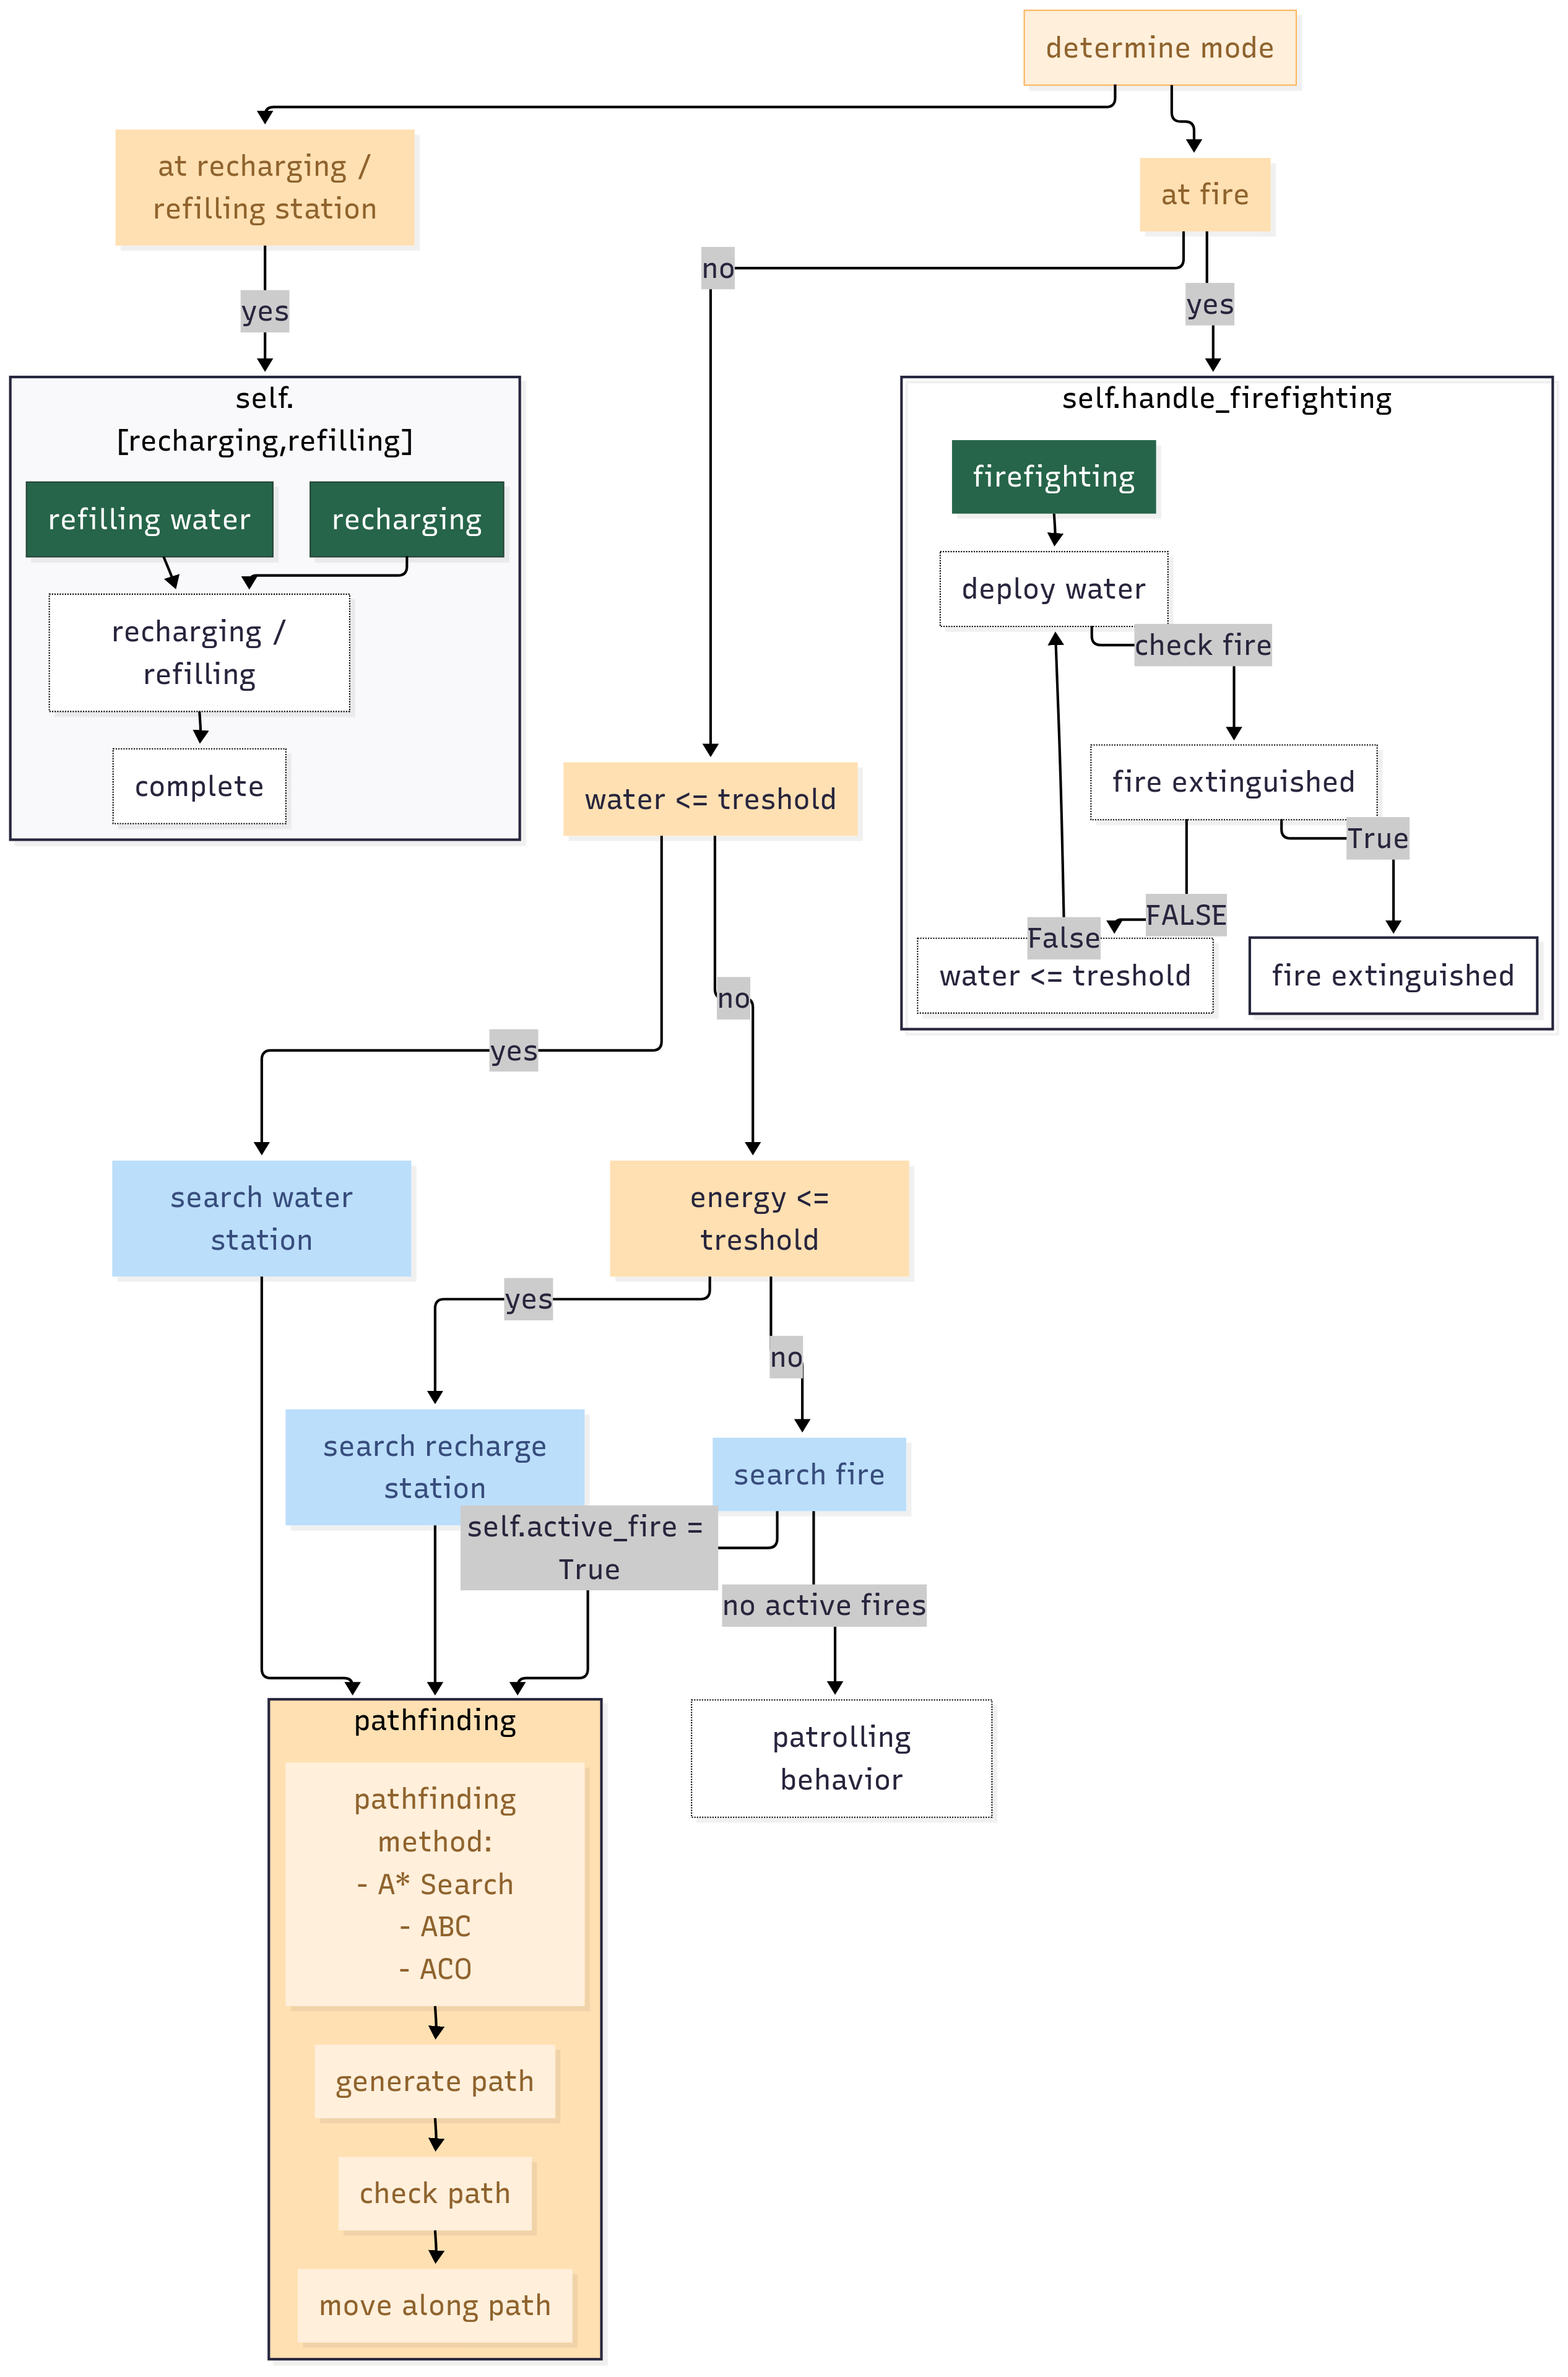
\includegraphics[width=0.8\textwidth]{figures/DroneAgent_Logic.png}
  \caption{Drone Agent Decision-Making Logic}
  \label{fig:droneAgentlogic}
\end{figure}

\newpage
\subsubsection{Firefighting Plane}
\label{sec:PlaneAgent}

The simulation framework incorporates manned aircraft as a benchmark to evaluate drone-based firefighting solutions. The Lockheed Martin C-130 Hercules was chosen as the reference platform due to its proven operational history, widespread use in aerial firefighting, and well-documented performance characteristics \citep{LockheedC130Hercules2022}. As a repurposed military transport aircraft, the C-130 represents a conventional approach to wildfire management, providing a solid baseline for assessing the effectiveness of emerging drone-based strategies. Due to its military design heritage it offers the capability to carry heavy payloads and has proven itself in reliability.
The C-130 aircraft, used as a reference for the firefighting plane, has an estimated range of \SI{2047}{\nauticalmile} = \SI{3791}{\kilo\meter} with max payload and \SI{4522}{\nauticalmile} = \SI{8375}{\kilo\meter} with an empty payload \citep{LockheedC130Hercules2022}. Considering simplicity the simulation assumes an average range of \SI{6000}{\kilo\meter} given the fact that the Plane is full and empty based on whether the water was dropped or is being delivered to the fire site. Considering these metrics a fuel consumption of \SI{6}{\liter}/km is calculated.
\[
\text{Fuel Consumption per km} =\frac{36000~\text{L}}{6000~\text{km}} = 6~\text{L/km}
\]

Given that the drone has a speed of 1 field per step which accounts for 36 km/h \citep{DJIAGRAST50} (equivalent to 10~m/s). Therefore, the speed of the plane needs to be normalized. In comparison, the C-130 has a cruising speed of 600 ~km/h \citep{LockheedC130Hercules2022} (or 167~m/s), considering that the speed for firefighting is significantly lower a speed of 250~km/h \ (\(\approx 69.4~\text{m/s}\)) is chosen resulting in a relative speed factor of:

\begin{equation}
\text{Speed Factor}= \frac{70~\text{m/s}}{10~\text{m/s}} = 7
\end{equation}

Therefore, the speed of the plane is defined by the value 7 (positions per step)
This factor is used to scale operational parameters when comparing drone and plane behavior within the simulation. To calculate the fuel consumption with a speed of 250~\text{km/h} \ (\(\approx 69.4~\text{m/s}\)), and simulation steps defined as 1-second intervals:

\[
\text{Fuel Consumption per Step}= (6~\text{L/km}) \times \frac{250}{3600}~\text{km/s} = 0.417\text{ L/step}
\]

The emission rate of the firefighting plane is based on data from \citet*{spicerRapidMeasurementEmissions2009}, which reports an emission of approximately \SI{0.3073}{\kilo\gram} CO\textsubscript{2} for every kilogram of fuel consumed assuming Jet-A fuel with a density of 0.8~kg/L. The emission per step is calculated as follows: 
\[
\text{Emission per Liter}  = 0.3073~\frac{\text{kg CO}_2}{\text{kg fuel}} \times 0.8~\frac{\text{kg fuel}}{\text{L}} = 0.24584~\frac{\text{kg CO}_2}{\text{L}}
\]

\[
\text{Emissions per Step} = 0.417~\text{L/step} \times 0.24584~\frac{\text{kg CO}_2}{\text{L}} = 0.1025~\text{kg CO}_2/\text{step}
\]


As stated by \citet*{spicerRapidMeasurementEmissions2009} is it important to point out that the emissions fluctuate significantly depending on cruising speed and weather conditions. For simplicity reasons the emissions per step are a fixed parameter calculated as mentioned.

In addition to similar parameters, the logic of the plane also works differently. A key difference is the plane specific interaction with the Runway class, simulating refueling, takeoff and landing behavior. A key difference between the Plane and Drone class is its characteristic behavior; the drone has a smaller turning radius and is able to refuel from the resource stations autonomously, whereas the plane is dependent on a runway in order to refuel water and fuel. In addition, the emissions are expected to be much higher because it runs on fossil fuels and not electricity. However, the plane moves faster and has a higher water loading capacity which enables it in theory to extinguish fires faster. 



%TC:ignore
\begin{center}
\begin{longtable}{>{\raggedright\arraybackslash}p{4.4cm} >{\raggedright\arraybackslash}p{1.4cm} >{\raggedright\arraybackslash}p{6.4cm}}
\caption{Firefighting Plane Class Parameters} \\
\toprule
\textbf{Parameter Name} & \textbf{Default Value} & \textbf{Description} \\
\midrule
\endfirsthead

\multicolumn{3}{c}%
{{\bfseries \tablename\ \thetable{} -- continued from previous page}} \\
\toprule
\textbf{Parameter Name} & \textbf{Default Value} & \textbf{Description} \\
\midrule
\endhead

\bottomrule
\multicolumn{3}{r}{{Continued on next page}} \\
\endfoot

\bottomrule
\endlastfoot

\multicolumn{3}{l}{\textbf{Basic Parameters}} \\
\midrule
unique\_id & int & Unique identifier for the plane agent \\
typ & ``plane'' & Agent type identifier \\
location & None & Current position of the plane \\
goal & None & Target destination \\
path & [list] & Calculated path to destination \\
speed & 7 & Movement cells per step \\
\midrule

\multicolumn{3}{l}{\textbf{Resource Parameters}} \\
\midrule
water\_capacity & \SI{18184}{\liter} & = 4000 gallons C-130 \citep{LockheedSuperHercules} \\
water & 2000 & Current water level \\
water\_threshold & 500 & Minimum water level before refill \\
water\_used & 0 & Total water used during operations \\
water\_drop\_rate & \SI{8.328}{\liter}/s &  = 2200 gallons/s C-130 aircraft \\

fuel\_capacity &  \SI{3600}{\liter} & = 9530 gallons  \citep{LockheedC130Hercules2022}\\
fuel & 1000 & Current fuel level \\
fuel\_threshold & 200 & Minimum fuel level before refueling\\
\midrule

\multicolumn{3}{l}{\textbf{Time and State Parameters}} \\
\midrule
refill\_time & 10 & Time steps required to refill water \\
refill\_time\_remaining & 0 & Countdown for current refill operation \\
refueling\_time\_remaining & 0 & Countdown for current refueling operation \\
refueling & T/F & Boolean indicating refueling state\\
time\_at\_fire & 0 & Time spent at current fire \\
max\_time\_at\_fire & 2 & Maximum time to spend at a fire \\
\midrule

\multicolumn{3}{l}{\textbf{Environmental Impact Parameters}} \\
\midrule
emission\_rate & 0.24584 & Kg CO\textsubscript{2} / L fuel \citep{spicerRapidMeasurementEmissions2009} \\ 
total\_emission & 0.0 & Cumulative emissions produced \\
operational\_cost\_per\_step & 0.5 & Base operational cost per step \\
fuel\_cost\_per\_unit & 0.1 & Cost per unit of fuel \\
total\_cost & 0.0 & Cumulative operational cost \\
\midrule

\multicolumn{3}{l}{\textbf{Target References}} \\
\midrule
current\_target & None & Current target object (fire, runway, etc.) \\
target\_fire & None & Reference to the specific fire being targeted \\
fires & [list] & List of all known fires \\
firefighting & T/F & Boolean indicating firefighting state \\
\label{fig:plane_parameters}
\end{longtable}
\end{center}
\newpage

\begin{figure}[H]
    \centering
    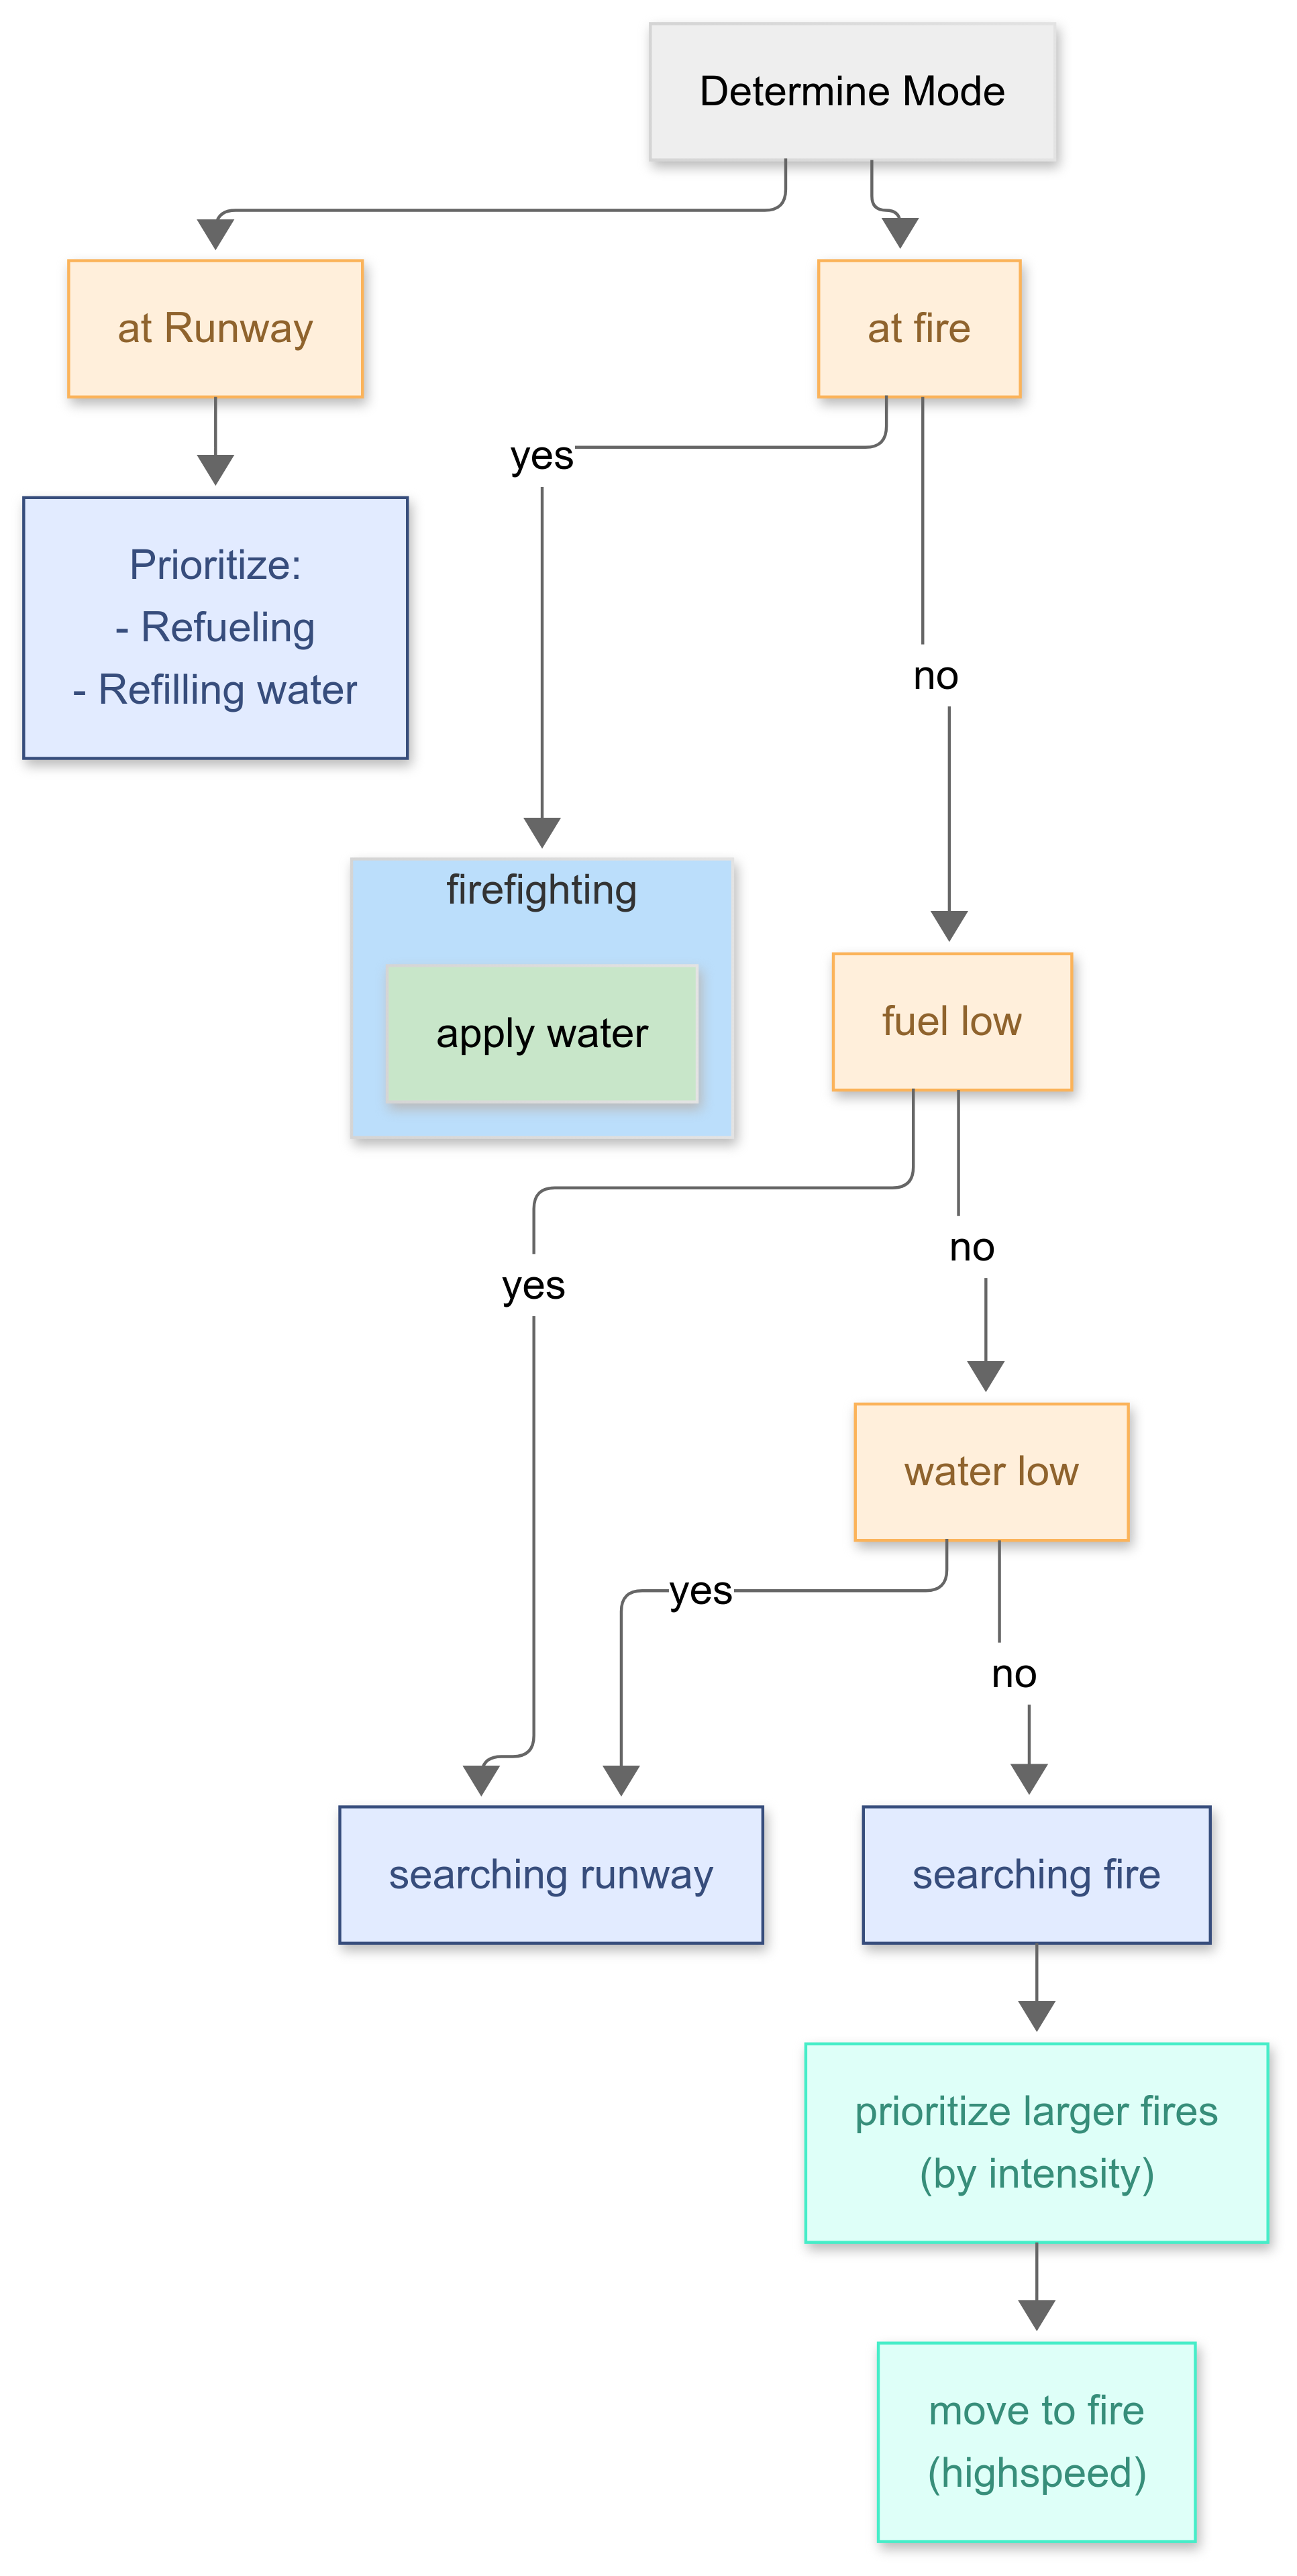
\includegraphics[width=0.6\linewidth]{figures/plane_logic.png}
    \caption{Plane Logic}
    \label{fig:planeLogic}
\end{figure}
\newpage

\subsubsection{Water Station}
\label{sec:WaterStation}
Water Stations are key infrastructure agents responsible for refilling the drone. Each station has a limited refill rate, introducing a time cost to each interaction. Water usage data per refill is collected for each agent, and the refill interaction contributes to total operational cost and emissions. Placement of Water Stations influences overall suppression efficiency and is therefore predefined to ensure comparability between approaches. The chosen parameters can be observed in Table~\ref{fig:waterStation}.

\subsubsection{Recharge Station}
\label{sec:RechargeStation}
Environmental sustainability represents a primary design consideration for the recharge station network. Each station's operations are characterized by an emissions factor of 0.200 kg CO\textsubscript{2} per kWh provided, based on research conducted by \citet*{stolaroffEnergyUseLife2018}, which compares energy efficiency of different drone delivery systems. It is important to highlight that emissions caused by green electricity generated through solar panels highly fluctuate and can range from ``40g to 180g of CO\textsubscript{2} per kWh for PV'' \citep{GreenhousegasEmissionsSolar2007}, depending on various factors. For simplicity reasons the value proposed by  \citet*{stolaroffEnergyUseLife2018} will be used to calculate emissions caused by the recharge station in connection with the drones. The electricity cost is based on the EU average of 2023 \citep{ElectricityPriceStatistics}, with a value of 0.2872 euro per kWh. \texttt{total\_energy\_provided} and \texttt{recharge\_event} are metrics to calculate the usage of the recharge station and can be used for more in-depth analytics. The chosen parameters are illustrated in Table~\ref{fig:rechargeStation}.

\subsubsection{Fire Agent}
\label{sec:FireAgent}

As this study is in the field of multiagent systems every instance in the simulation is an agent, therefore also the fire needs to be defined as an agent. As shown in Appendix~\ref{app:FireAgentParameters} the fire agent has customizable parameters which allow for complex interactions with the firefighting vehicles. To mimic the real world the fire agents spawn in the environment with different intensities and have the possibility to spread to a neighboring cell. The spread fire is its own agent with a slightly lower intensity. Through functions such as \texttt{apply\_water(water\_amount)} the fire agent receives water from the given firefighting agent and extinguishes. The parameters for the \texttt{FireAgent} can be observed in Appendix~\ref{app:FireAgentParameters}. When fire spreads to neighboring cells, new fire agents are created, meaning that a higher fire count reflects fire area growth rather than the ignition of new fires.

\subsubsection{Runway Agent}
\label{sec:RunwayClass}
The runway agent is created specifically for the firefighting plane. A plane needs a runway to start, takeoff and refill fuel and water, contradictory to a drone which can autonomously refill itself and charge itself through a given station. The runway is implemented to ensure a logical approach to real-world firefighting models. It is kept track of whether the runway is currently occupied to make sure multiple planes do not collide. The parameters of the runway class are explained in appendix~\ref{app:runway_parameters}

\subsection{Path-finding Algorithms}
Each drone selects paths using of one of the following algorithms:
\begin{enumerate}
    \item A* Search: Heuristic-based algorithm with low resource usage. Efficient for small or structured environments. Implemented through the \texttt{heapq} Python library \citep{python-heapq}.
    \item Artificial Bee Colony (ABC): Swarm-inspired, decentralized optimization method effective in dynamic or noisy spaces \citep{karaboga2007abc}.
    \item Ant Colony Optimization (ACO): Probabilistic method using pheromone trails to discover optimal paths over time \citep{ACO}.
\end{enumerate}

The same algorithm is used for all drones within a simulation run to ensure internal consistency. All algorithms are tested across otherwise identical parameters to evaluate comparative performance. These were selected based on experimentation and prior research.

\subsection{Data-Collection}

As mentioned earlier the Simulation is created with the SAT model in mind. Therefore, a robust and extensive Data-Collector model is needed. At every step every agent's properties are stored in the \texttt{agent\_data} data-frame and the models properties in the \texttt{model\_data} data-frame. This data collection is enabled through the \texttt{mesa.datacollection.DataCollector{}} which is part of the Mesa framework. \texttt{agent\_reporters} and \texttt{model\_reporters} make this function possible. Extensive details can be found in the \href{https://github.com/kaispeidel/Autonomous-Drone-Firefighting-Simulation}{GitHub repository}.

\subsection{Risk Assessment with Machine Learning}

To evaluate whether the simulation output could support future autonomous risk-based decision-making, two unsupervised learning methods were integrated: 
\begin{enumerate}
    \item DBSCAN \citep{dbscan}: A density-based clustering algorithm to identify spatial risk zones.
    \item K-Means \citep{kmeans}: A centroid-based algorithm to segment environments based on fire intensity and suppression delay.
\end{enumerate}

These algorithms were applied to the collected simulation data capturing fire intensity, suppression history, and spatial coordinates. The purpose was exploratory, testing whether simulated environments show meaningful emergent patterns that could later guide agent behavior. The main algorithms used was DBSCAN with falling back to K-Means if failing.

No hyperparameter tuning was performed due to the exploratory nature of the task; default \texttt{scikit-learn} parameters were used, with basic preprocessing (normalization and NaN filtering).

\subsection{Technical Implementation and Reproducibility}

\begin{enumerate}
    \item Language: Python 3.11 \citep{python3.11}
    \item Packages: Key packages include \texttt{mesa} \citep{terMesa}, \texttt{numpy} \citep{numpy}, \texttt{pandas} \citep{reback2020pandas}, \texttt{matplotlib} \citep{Matplotlib}, \texttt{seaborn} \citep{seaborn} , \texttt{heapq} \citep{python-heapq} \texttt{scikit-learn} \citep{scikit-learn}, an exhaustive list of all requirements are listed in the repository: (\texttt{see requirements.txt})
    \item Code repository: \href{https://github.com/kaispeidel/thesis}{AgentBasedFirefightingModel\_repository} \citep{AgentBasedFirefightingModel_repository}
\end{enumerate}

The entire simulation is designed to be reproducible and configurable. All agent parameters, environment size, and algorithm settings can be controlled via parameters.


\section{Results}
\section{Discussion}

\appendix
%ModelLogic
\label{app:modellogic}

\begin{figure}[H]
    \centering
    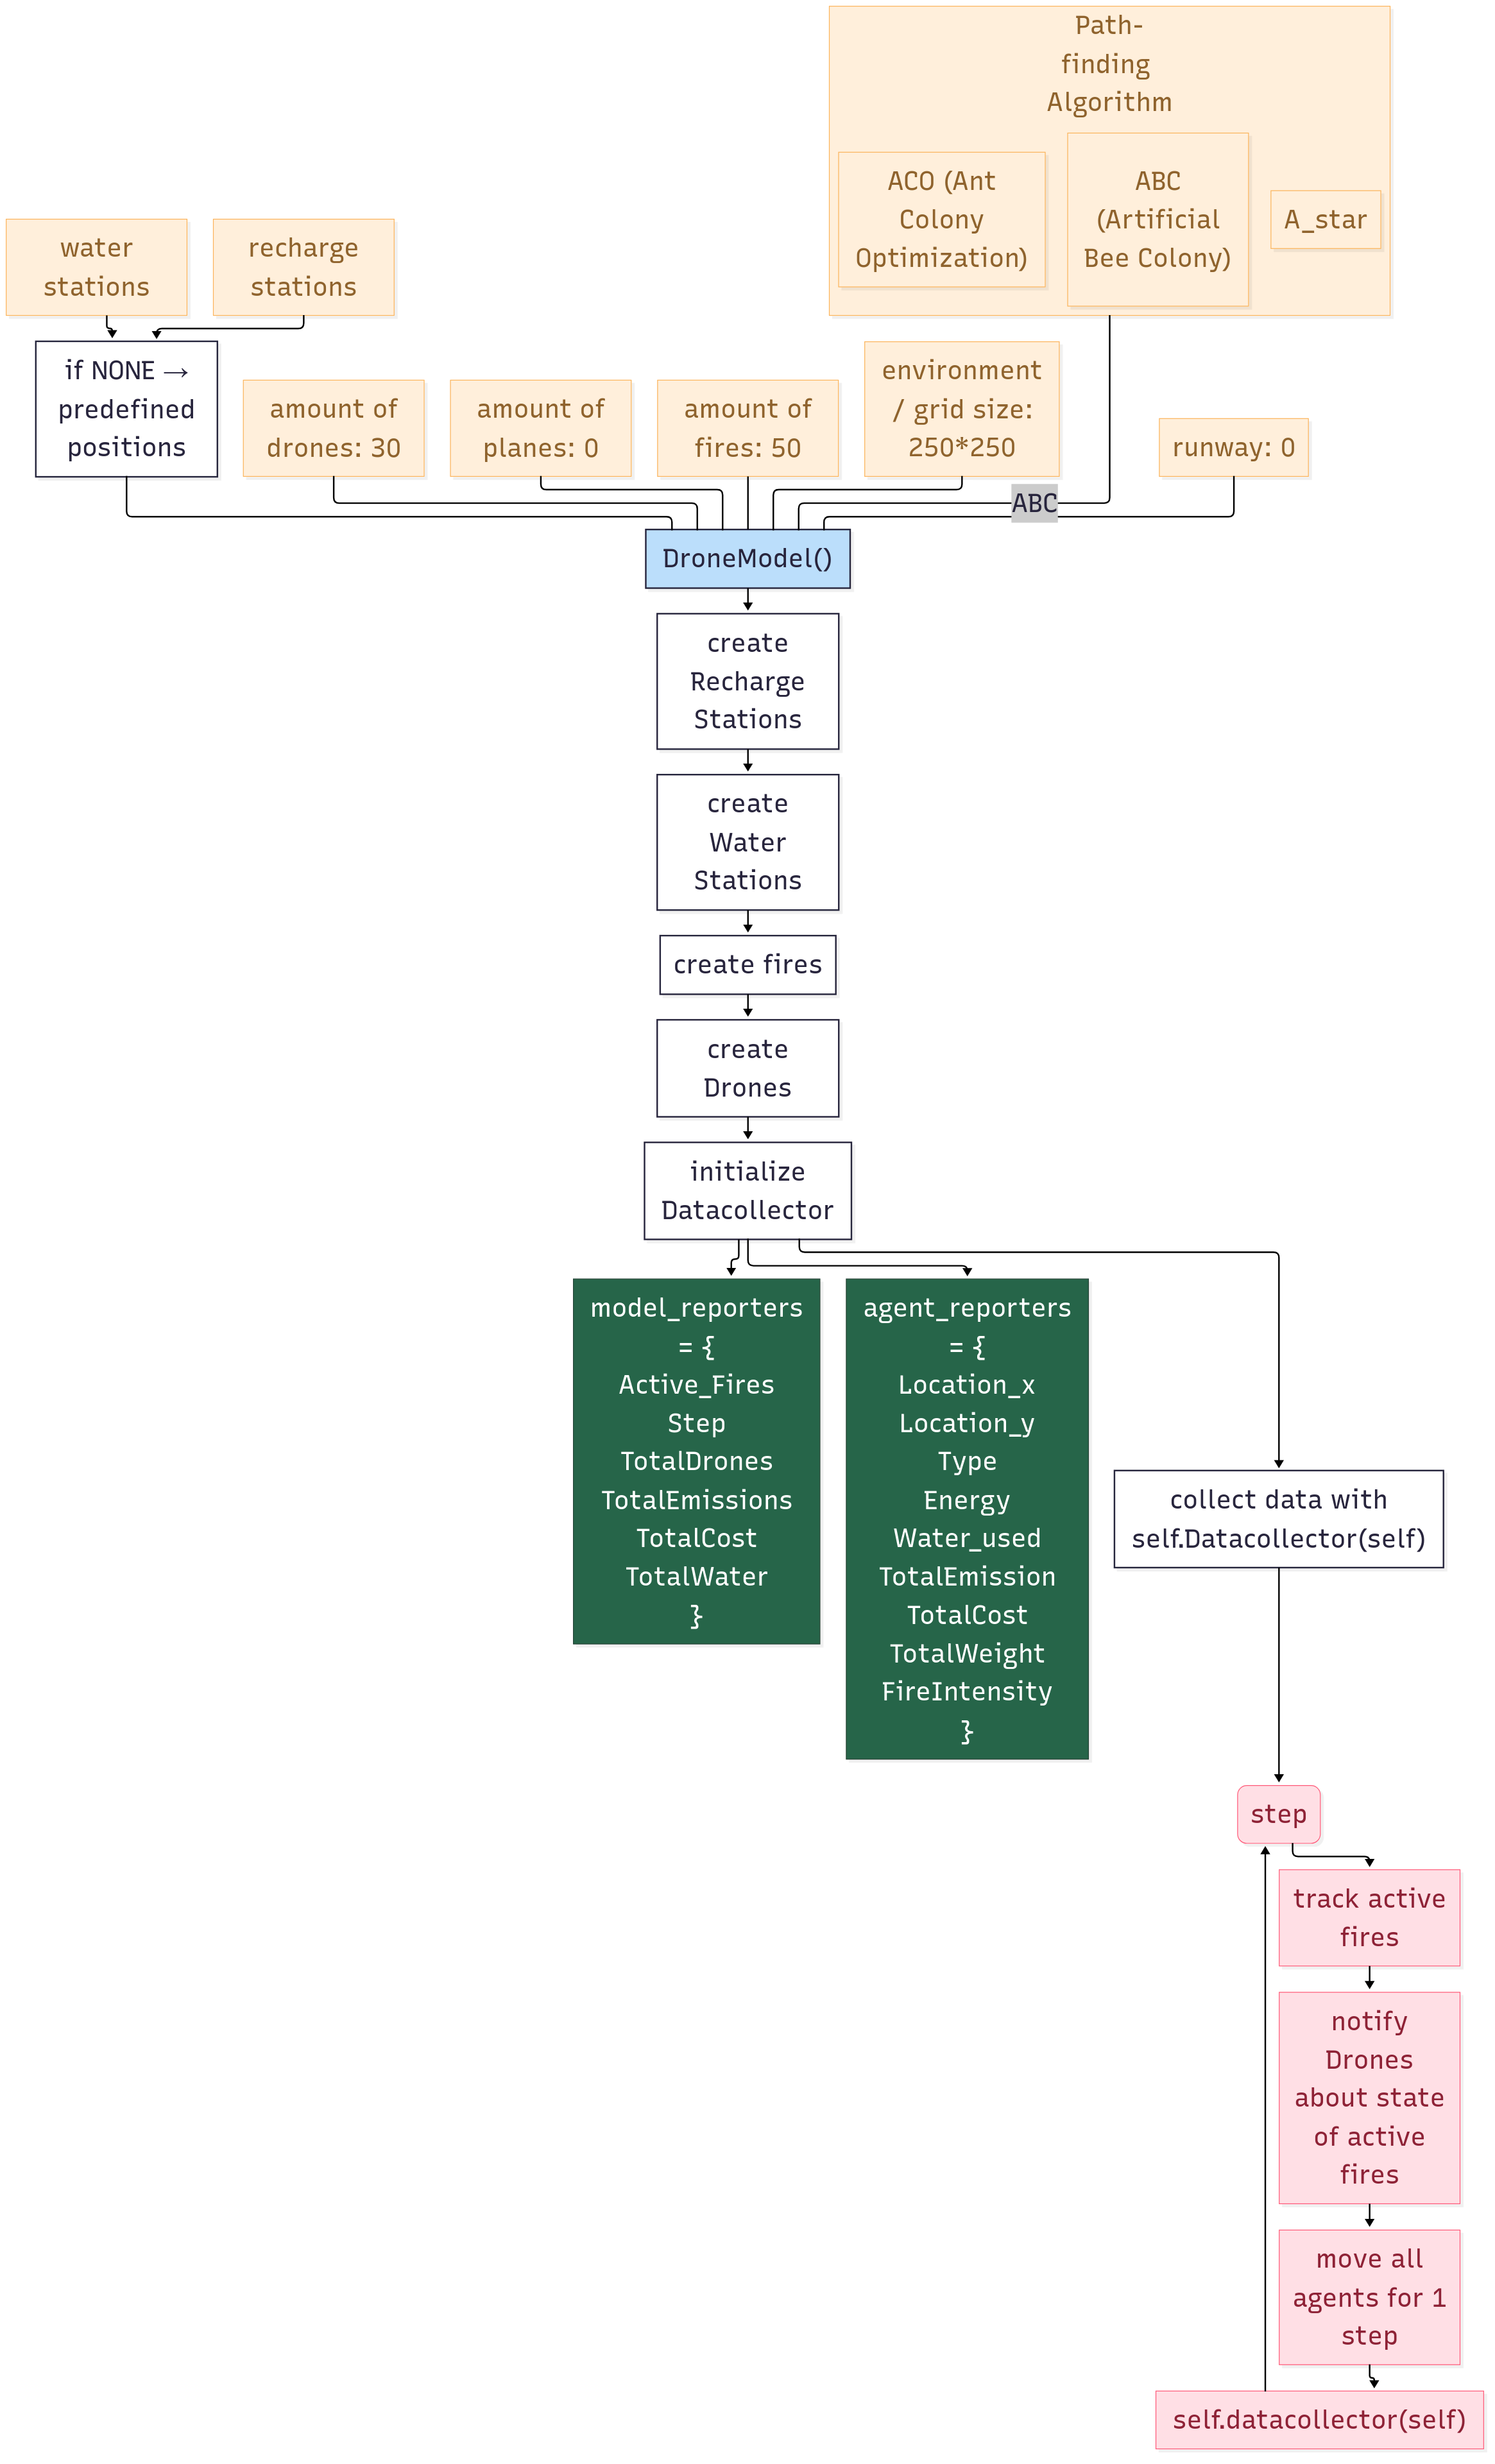
\includegraphics[width=0.7\textwidth]{figures/modellogic.png}
    \caption{Complete Model Architecture and Agent Interaction Logic}
    \label{fig:modellogic}
\end{figure}

%Water Station
\begin{center}
\begin{longtable}{>{\raggedright\arraybackslash}p{4.4cm} >{\raggedright\arraybackslash}p{1.4cm} >{\raggedright\arraybackslash}p{6.4cm}}
\caption{Water Station Agent Parameters} \label{fig:waterStation} \\
\toprule
\textbf{Parameter Name} & \textbf{Default Value} & \textbf{Description} \\
\midrule
\endfirsthead

\multicolumn{3}{c}%
{{\bfseries \tablename\ \thetable{} -- continued from previous page}} \\
\toprule
\textbf{Parameter Name} & \textbf{Default Value} & \textbf{Description} \\
\midrule
\endhead

\bottomrule
\multicolumn{3}{r}{{Continued on next page}} \\
\endfoot

\bottomrule
\endlastfoot

\multicolumn{3}{l}{\textbf{Initialization Parameters}} \\
\midrule
location & [x,y] & Position of the water station \\
capacity & \SI{1000}{\liter} & Maximum water capacity in liters \\
unique\_id & int & Unique identifier for the agent \\
typ & ``water\_station'' &  \\
active & T/F & Boolean indicating operational status \\
\midrule

\multicolumn{3}{l}{\textbf{Operational Parameters}} \\
\midrule
refill\_rate & \SI{20}{\liter} & Water refilled automatically per step \\
\midrule

multicolumn{3}{l}{\textbf{Environmental Impact}} \\
\midrule
emissions\_factor & 0.20 & Emissions in kg of CO\textsubscript{2} per liter dispensed \\
total\_emissions & 0.0 & Total emissions accumulated \\
\midrule

\multicolumn{3}{l}{\textbf{Cost Metrics}} \\
water\_cost & €0.00061 & Cost per liter of water: Given €0.6 per m\textsuperscript{3} equals to 0.00061€ per liter \citep{waterPricing} \\
maintenance\_cost & €0.03 & Fixed operating cost per step \\
total\_cost & €0.0 & Cumulative cost of operations \\
\midrule

\multicolumn{3}{l}{\textbf{Usage Metrics}} \\
\midrule
total\_water\_provided & \SI{0}{\liter} & Total liters of water provided \\
refill\_events & 0 & Accumulated number of refill events \\

\end{longtable}
\end{center}


%recharge Station
\begin{center}
\begin{longtable}{>{\raggedright\arraybackslash}p{4.4cm} >{\raggedright\arraybackslash}p{1.4cm} >{\raggedright\arraybackslash}p{6.4cm}}
\caption{Recharge Station Agent Parameters} \label{fig:rechargeStation} \\
\toprule
\textbf{Parameter Name} & \textbf{Default Value} & \textbf{Description} \\
\midrule
\endfirsthead

\multicolumn{3}{c}%
{{\bfseries \tablename\ \thetable{} -- continued from previous page}} \\
\toprule
\textbf{Parameter Name} & \textbf{Default Value} & \textbf{Description} \\
\midrule
\endhead


\bottomrule
\multicolumn{3}{r}{{Continued on next page}} \\
\endfoot

\bottomrule
\endlastfoot

\multicolumn{3}{l}{\textbf{Initialization Parameters}} \\
\midrule
location & [x,y] & Position of the recharge station \\
unique\_id & int & Unique identifier for the agent \\
typ & ``recharge\_station'' &  \\
active & T/F & Boolean indicating active status \\
\midrule

\multicolumn{3}{l}{\textbf{Operational Parameters}} \\
\midrule
charge\_rate & 100 & Energy units provided per recharge step \\
\midrule

\multicolumn{3}{l}{\textbf{Environmental Impact}} \\
\midrule
emissions\_factor & 0.200 & Emissions in kg of CO\textsubscript{2} per kWh provided. The energy emission varies based on a various factors. The given value is based on a research done by \citet*{stolaroffEnergyUseLife2018} which shows energy emission efficiency in drones.\\
total\_emissions & 0.0 & Total emissions accumulated \\
\midrule

\multicolumn{3}{l}{\textbf{Cost Metrics}} \\
\midrule
electricity\_cost & €0.2872 & Electricity cost per kWh taken from the EU average in 2023 \citep{ElectricityPriceStatistics}. \\
maintenance\_cost & €0.05 & Fixed operational cost per step \\
total\_cost & €0.0 & Total operational cost accumulated \\
\midrule

\multicolumn{3}{l}{\textbf{Usage Metrics}} \\
\midrule
total\_energy\_provided & 0.0 & Total kWh of energy provided \\
recharge\_events & 0 & Accumulated number of recharge events \\

\end{longtable}
\end{center}






%FireAgent
\begin{center}
\begin{longtable}{>{\raggedright\arraybackslash}p{4.4cm} >{\raggedright\arraybackslash}p{1.4cm} >{\raggedright\arraybackslash}p{6.4cm}}
\caption{Fire Agent Parameters} \label{app:FireAgentParameters} \\
\toprule
\textbf{Parameter Name} & \textbf{Default Value} & \textbf{Description} \\
\midrule
\endfirsthead

\multicolumn{3}{c}%
{{\bfseries \tablename\ \thetable{} -- continued from previous page}} \\
\toprule
\textbf{Parameter Name} & \textbf{Default Value} & \textbf{Description} \\
\midrule
\endhead

\bottomrule
\multicolumn{3}{r}{{Continued on next page}} \\
\endfoot

\bottomrule
\endlastfoot

\multicolumn{3}{l}{\textbf{Initialization Parameters}} \\
\midrule
location & [x,y] &  Coordinates of the fire area \\
intensity & 5 & Fire intensity on a scale from 1 to 10 \\
size & 1 & Size of the fire (radius) \\
unique\_id & int & Unique identifier for the agent \\
typ & "fire" & Type identifier for the agent \\
active & T/F & Boolean indicating whether the fire is currently burning \\
age & 0 & Age of the fire in simulation steps \\
water\_applied & 0 & Total water applied to this fire \\
\midrule

\multicolumn{3}{l}{\textbf{Spreading Behavior}} \\
\midrule
spread\_probability & 0.05 & Base chance of spreading per step \\
last\_spread\_attempt & 0 & Step count of last spread attempt \\
spread\_cooldown & 10 & Minimum steps between spread attempts \\
\midrule

\multicolumn{3}{l}{\textbf{Methods and Behaviors}} \\
\midrule
apply\_water(water\_amount) & — & Reduces intensity, extinguishes fire if intensity $\leq 0.5$ \\
step() & — & Ages fire, increases intensity slightly, attempts spread \\
attempt\_spread() & — & Checks for nearby cells and spreads if possible \\
extinguish() & — & Manually sets fire as extinguished \\

\end{longtable}
\end{center}

%Runwayparameters
\begin{center}
\begin{longtable}{>{\raggedright\arraybackslash}p{4.4cm} >{\raggedright\arraybackslash}p{1.4cm} >{\raggedright\arraybackslash}p{6.4cm}}
\caption{Runway Agent Parameters} \label{app:runway_parameters} \\
\toprule
\textbf{Parameter Name} & \textbf{Default Value} & \textbf{Description} \\
\midrule
\endfirsthead

\multicolumn{3}{l}{\textbf{Initialization Parameters}} \\
\midrule
location & [x,y] & Grid location of the runway \\
typ & ``runway'' & Type identifier for the agent \\
is\_occupied & T/F & Boolean indicating occupancy status \\
occupying\_plane & None & Reference to the plane currently on the runway \\
\midrule

\multicolumn{3}{l}{\textbf{Resource Capacities}} \\
\midrule
fuel\_capacity & \SI{10000}{\liter} & Maximum amount of fuel the runway can store \\
fuel\_level & \SI{10000}{\liter} & Current fuel level in the runway \\
water\_capacity & \SI{20000}{\liter} & Maximum amount of water the runway can store \\
water\_level & \SI{20000}{\liter} & Current water level in the runway \\
\midrule

\multicolumn{3}{l}{\textbf{Refill Rates (Per Step)}} \\
\midrule
fuel\_refill\_rate & \SI{200}{\liter} & Fuel replenished per simulation step \\
water\_refill\_rate & \SI{500}{\liter} & Water replenished per simulation step \\
\midrule

\multicolumn{3}{l}{\textbf{Environmental Impact Parameters}} \\
\midrule
fuel\_emissions\_factor & 0.2 kg & CO\textsubscript{2} emissions per unit of fuel provided \\
water\_emissions\_factor & 0.1 kg & CO\textsubscript{2} emissions per unit of water provided \\
total\_emissions & 0.0 kg & Cumulative emissions generated \\
\midrule

\multicolumn{3}{l}{\textbf{Cost Parameters}} \\
\midrule
fuel\_cost & €0.3 & Cost per unit of fuel provided \\
water\_cost & €0.05 & Cost per unit of water provided \\
maintenance\_cost & €0.5 & Operational maintenance cost per step \\
total\_cost & €0.0 & Accumulated operational costs \\
\midrule

\multicolumn{3}{l}{\textbf{Usage Statistics}} \\
\midrule
planes\_serviced & 0 & Total number of planes serviced \\
fuel\_provided & 0.0 & Total fuel supplied to planes \\
water\_provided & 0.0 & Total water supplied to planes \\

\end{longtable}
\end{center}


\bibliographystyle{apalike}
\bibliography{references}

\end{document}